% \chapter{Methoden und Praktiken}

\textit{In diesem Kapitel soll beschrieben werden, wie eine Nachvollziehbarkeit in Webapplikationen erreicht werden kann. Spezielle Methoden und Praktiken sollen vorgestellt und beleuchtet werden.}
% \textit{Hier könnte unter anderem \textbf{OpenTelemetry} betrachtet werden.}

\section{Methoden}

\subsection{Logging}

\textit{Folgende Fragen sollen zur Methode beantwortet werden}
\begin{enumerate}
	\item \textit{Gibt es Besonderheiten zu Logging in anderen Projekten (Backend vs. Frontend)?}
	\item \textit{Wie können Logs an einen auswertenden Stakeholder gelangen??}
	\item \textit{Welches Verhalten kann hiermit aufgedeckt/nachvollziehbar gemacht werden?}
\end{enumerate}

%\subsection{Monitoring}
%
%\textit{Folgende Fragen sollen zur Methode beantwortet werden}
%\begin{enumerate}
%	\item \textit{Welche Anwendungseigenschaften sind zu monitoren?}
%	\item \textit{Welches Verhalten kann hiermit aufgedeckt/nachvollziehbar gemacht werden?}
%\end{enumerate}

\subsection{Metriken}

\textit{Folgende Fragen sollen zur Methode beantwortet werden}
\begin{enumerate}
	\item \textit{Welche Metriken können definiert?}
	\item \textit{Wie können Metriken definiert werden?}
	\item \textit{Welches Verhalten kann hiermit aufgedeckt/nachvollziehbar gemacht werden?}
\end{enumerate}

\subsection{Tracing}

\textit{Folgende Fragen sollen zur Methode beantwortet werden}
\begin{enumerate}
	\item \textit{Welche Nutzerinteraktionen sind zu tracen?}
	\item \textit{Welches Verhalten kann hiermit aufgedeckt/nachvollziehbar gemacht werden?}
\end{enumerate}

\subsection{Fehlerberichte}

\textit{Folgende Fragen sollen zur Methode beantwortet werden}
\begin{enumerate}
	\item \textit{Was genau sind Fehlerberichte (=Bug-Reports) }
	\item \textit{Welches Verhalten kann hiermit aufgedeckt/nachvollziehbar gemacht werden?}
\end{enumerate}

\section{Werkzeuge und Technologien}

%\textit{Basierend auf dem Grundwissen über die Methoden und Praktiken, soll nun der Stand der Technik erörtert werden. Hierbei sollen Werkzeuge und Technologien und ihre Ansätze hervorgehoben werden und mit Hilfe welcher Methoden sie welches Ziel erreichen.}
%
%\textit{Wie in der Zielsetzung definiert sollen hier zwei bis drei Technologien näher vorgestellt werden.}
%
%\textit{Weiterhin könnte beleuchtet werden, wie ähnliche Herausforderungen bei anderen „Fat-Client“-Lösungen (also nicht SPAs) angegangen werden, und kann man hier vielleicht etwas lernen oder übertragen (und wenn nicht, warum nicht)?}

In der Fachpraxis haben sich einige Technologien über die Jahre entwickelt und etabliert, die eine verbesserte Nachvollziehbarkeit als Ziel haben. Es lassen sich zudem verschiedene Funktionskategorien festlegen, auf die sich die jeweiligen Technologien konzentrieren. Die einzelnen Technologien lassen sich jedoch nicht strikt kategorisieren und weisen unterschiedliche Funktionsumfänge für dieselben Kategorien auf. Deshalb werden die Kategorien folgend beschrieben, aber bei der Vorstellung der Technologien erfolgt keine Kategorisierung oder direkte Gegenüberstellung.

\subsection{Kategorien}

\subsubsection{System Monitoring}

System Monitoring beschäftigt sich mit der Überwachung der notwendigen Systeme und Dienste in Bezug auf Hardware- und Softwareressourcen. Es handelt sich hierbei um ein projektunabhängiges Monitoring, welches sicherstellen soll, dass die Infrastruktur funktionstüchtig bleibt.

\subsubsection{Log Management}

Log Management umfasst die Erfassung, Speicherung, Verarbeitung und Analyse von Logdaten von Anwendungen. Weiterhin bieten Werkzeuge hierbei oftmals Such- und Meldefunktionen.

\subsubsection{Application Performance Monitoring (APM)}

Beim Application Performance Monitoring werden Daten innerhalb von Applikationen gesammelt, die Rückschlüsse auf die Perfomanz von bspw. Transaktionen geben sollen \cite{StudyingTheEffectivenessOfAPMTools}. Mit diesen Daten können dann Regressionen der Performanz, in Aspekten wie Zeitaufwand oder Ressourcennutzung, festgestellt werden.

\subsubsection{Real User Monitoring (RUM)}

Real User Monitoring beschäftigt sich mit dem Mitschneiden von allen Nutzerinteraktionen mit bspw. einer Webapplikation. Hiermit lässt sich nachvollziehen, wie ein Nutzer die Anwendung verwednet. RUM kann dazu verwendet werden um Herauszufinden, wie ein Nutzer zu einem Zustand gelangt ist. Aber es können auch ineffiziente Klickpfade hierdurch festgestellt werden und darauf basierend UX Verbesserungen vorgenommen werden.

\subsubsection{Synthetic Monitoring}

Beim Synthetic Monitoring werden Endnutzerszenarien simuliert, um zu prüfen und sicherzustellen, dass diese Szenarien wie gewünscht ablaufen. Hierbei kann auf Aspekte wie Funktionalität, Verfügbarkeit und auch verstrichene Zeit kontrolliert werden.

\subsubsection{Tracing}

Tracing beschäftigt sich mit dem Aufzeichnen von Kommunikationsflüssen. Hierbei können einerseits die Kommunikationsflüsse innerhalb einer Applikation oder innerhalb eines Systems erfasst werden, aber auch andererseits die Kommunikationsflüsse bei verteilten Systemen erfasst werden, um diese meist komplexen Zusammenhänge zu veranschaulichen. Ein herstellerunabhängiger Standard, der sich aus diesem Gebiet entwickelt hat, ist OpenTracing \cite{OpenTracing}.

\subsubsection{Error/Crash Monitoring}

Das Error Monitoring konzentriert sich auf das Erfassen und Melden von Fehlern. Es werden oftmals neben dem eigentlichen Fehler auch Aspekte vom RUM und Logging gemeldet, um mehr Kontextinformationen zu liefern.

\subsubsection{Session Replay}

Session Replay bedeuted, dass eine Sitzung eines Nutzers nachgestellt wird, so als ob sie gerade passiert. Hierbei können einzelne Aspekte der Anwendung nachgestellt werden, bspw. der Kommunikationsablauf, bei dem die tatsächliche zeitliche Abfolge von Kommunikationen nachvollzogen werden können. Desto mehr Aspekte nachgestellt werden, desto realitätsnaher ist die Simulation und entsprechend hilfreich ist sie beim Nachvollziehen.

\subsection{Fachpraxis}

\subsubsection{OpenTelemetry}

\begin{wrapfigure}[20]{r}{0.45\textwidth}
\centering
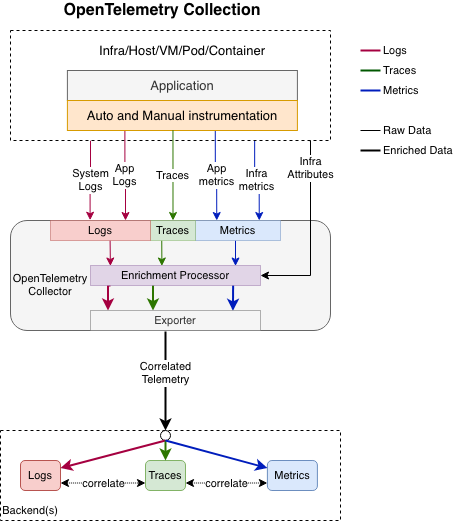
\includegraphics[width=\linewidth]{img/03_methoden/otel_unified-collection.png}
\caption{Schaubild einer Lösung auf Basis von OTel \cite{OpenTelemetryUnifiedCollection}}
\label{fig:otel-unified-collection}
\end{wrapfigure}

OpenTelemetry (OTel) \cite{OpenTelemetry} ist ein sich derzeit entwickelnder herstellerunabhängiger Standard, um Tracing-, Metrik- und Logdaten\footnotemark zu erfassen, verarbeiten, analysieren und zu visualisieren. Der Standard fasst die beiden Standards OpenTracing und OpenCensus \cite{OpenCensus} zusammen und hat sich als Ziel gesetzt diese zu erweitern. Hinter dem Standard stehen u. A. die Cloud Native Computing Foundation (CNCF), Google, Microsoft, und führende Hersteller in Tracing und Monitoring-Lösungen. Ein erster Release ist für Ende 2020/Anfang 2021 geplant. Ziel ist es, dass Entwickler Tools und Werkzeuge benutzen können, ohne jedesmal eine hochspezifische Anbindung schreiben und konfigurieren zu müssen. Stattdessen definiert der Standard Komponenten, die spezielle Aufgabengebiete haben und mit einer allgemeinen API angesprochen werden können. Die technische Infrastruktur einer Lösung basierend auf OTel kann in \autoref{fig:otel-unified-collection} betrachtet werden. Im groben definiert OTel folgende Komponenten: API, SDK, Exporter, Collector, Backend (vgl. \autoref{fig:otel-components}).

\begin{figure}[H]
	\centering
	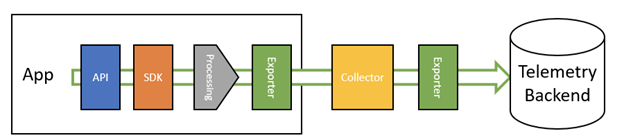
\includegraphics[width=0.75\linewidth]{img/03_methoden/dynatrace_otel-components.png}
	\caption{OTel Komponenten \cite{DynatraceOTelComponents}}
	\label{fig:otel-components}
\end{figure}

\nomenclature[Fachbegriff]{OTel}{OpenTelemetry}
\nomenclature[Fachbegriff]{CNCF}{Cloud Native Computing Foundation}
\footnotetext{Logging wird derzeit noch nicht unterstützt, es wird jedoch daran gearbeitet \cite{OpenTelemetryLoggingSpecification}}

\subsubsection{New Relic}

New Relic \cite{NewRelic} ist ein Dienst der gleichnamigen Firma, welcher Betreiber von Softwareprojekten dabei unterstützt das Verhalten ihrer Anwendungen zu überwachen. Der Dienst konzentriert sich auf System Monitoring, APM und RUM und erfasst die notwendigen Daten mit proprietären Lösungen. Neben den Kernfunktionalitäten unterstützt New Relic auch Log Management, Synthetic Monitoring, Tracing und Error Monitoring.

New Relic gibt an, dass Daten nach dem OpenTelemetry Standard selber erfasst und an New Relic gesendet werden können, ohne eine proprietäre Software \cite{NewRelicAnnoundOTelBetaSupport}. Leider ist dieses Feature in der Testversion, die zum evaluieren benutzt wurde, nicht enthalten und kann somit nicht bestätigt werden. Es sind jedoch offizielle und quelloffen veröffentlichte Exporter für New Relic verfügbar für .NET, Python und Java \cite{OpenTelemetryRegistry}.

\subsubsection{Dynatrace}

Dynatrace \cite{Dynatrace} ist ein Dienst der gleichnamigen Firma, welcher Betreiber von Softwareprojekten dabei unterstützt das Verhalten ihrer Anwendungen zu überwachen. Der Dienst konzentriert sich auf System Monitoring, APM und RUM und erfasst die notwendigen Daten mit proprietären Lösungen, dem OneAgent. Ganz ähnlich wie New Relic unterstützt Dynatrace neben den Kernfunktionalitäten auch Log Management, Synthetic Monitoring, Tracing und Error Monitoring.

Dynatrace ist dem OpenTelemetry Team beigetreten und hat angegeben, an der Weiterentwicklung mitzuhelfen \cite{DynatraceJoinOTelProject}. Eine Integration des Dienstes Dynatrace ins Ökosystem von OTel gibt es jedoch noch nicht.

\subsubsection{Sentry}

{\color{red}\textit{Beschreibung zu grundlegenden Eigenschaften von Sentry}}

\subsubsection{Splunk}

{\color{red}\textit{Beschreibung zu grundlegenden Eigenschaften von Splunk}}

\subsubsection{LogRocket}

{\color{red}\textit{Beschreibung zu grundlegenden Eigenschaften von LogRocket}}

\subsubsection{Honeycomb}

{\color{red}\textit{Beschreibung zu grundlegenden Eigenschaften von Honeycomb}}

\subsubsection{Jaeger}

Jaeger wurde 2017 als ein Projekt der CNCF gestartet \cite{Jaeger}. Es ist ein System für verteiltes Tracing von der Datensammlung bis hin zur Visualisierung, es unterstützt und implementiert den Standard OpenTracing.  Eine Unterstützung des OpenTelemetry Standards ist derzeit im Gange. Weiterhin kann Jaeger dazu benutzt werden, Metriken nach Prometheus \cite{Prometheus} zu exportieren, einem weiteren CNCF Projekt zur Speicherung und Visualisierung von Daten.

\subsubsection{Weiteres}

Bei meiner Recherche und Evaluierung wurden nicht alle auf dem Markt verfügbaren Werkzeuge und Technologien tiefergehend betrachtet. Deshalb werden weitere Funde, die nicht betrachtet wurden, hier kurz notiert:

\begin{itemize}
	\item APM \& RUM: AppDynamics, DataDog
	\item Error Monitoring: Airbrake, Instabug, Rollbar, Bugsnag, TrackJS
	\item Tracing: Google Cloud Trace, Zipkin
\end{itemize}

Auch diese Auflistung stellt nicht die komplette Bandbreite an Werkzeugen und Technologien dar und eine vorherige Betrachtung ist nicht als direkte Empfehlung zu verstehen.

\subsection{Literatur}